\section{Analisi dati: secondo set}
\subsection{Pressione e temperatura}

\begin{table}[H]
\centering

	\begin{subtable}{.5\textwidth}
		\centering
		\begin{tabular}{|c|c|} \hline
			\textbf{$\Delta h {[cm]}$ } & \textbf{T {[\degree C]} }  \\ \hline
			-0.5 & 0  \\ \hline
			18.3 & 4.7  \\ \hline
			30.4 & 7.77  \\ \hline
			43.4 & 11.5  \\ \hline
			57.9 & 15.1  \\ \hline
			69 & 18.1  \\ \hline
			76.6 & 20  \\ \hline
		\end{tabular}
		\caption{Aumento della temperatura}
	\end{subtable}%
	\begin{subtable}{.5\textwidth}
	\centering
	\begin{tabular}{|c|c|} \hline
		\textbf{$\Delta h {[cm]}$ } & \textbf{T {[\degree C]} }  \\ \hline
		76.6 & 20  \\ \hline
		58.7 & 15  \\ \hline
		49.6 & 12.5  \\ \hline
		35 & 8.7  \\ \hline
		19.9 & 5.1  \\ \hline
		-0.2 & 0.16  \\ \hline
	\end{tabular}
	\caption{Diminuzione della temperatura}
\end{subtable}

\caption{Dislivello $\Delta h$ in funzione della temperatura $T$}
\end{table}
In Tabella 1.a e Tabella 1.b troviamo riportati i dati raccolti durante la nostra esperienza rispettivamente aumentando e diminuendo la temperatura del bagno termico. 
Notiamo che l'ultimo valore della Tabella 1.a è uguale al primo valore della Tabella 1.b.
Troviamo graficati tali dati in Figura 1. 

\begin{figure}[H]
\centering
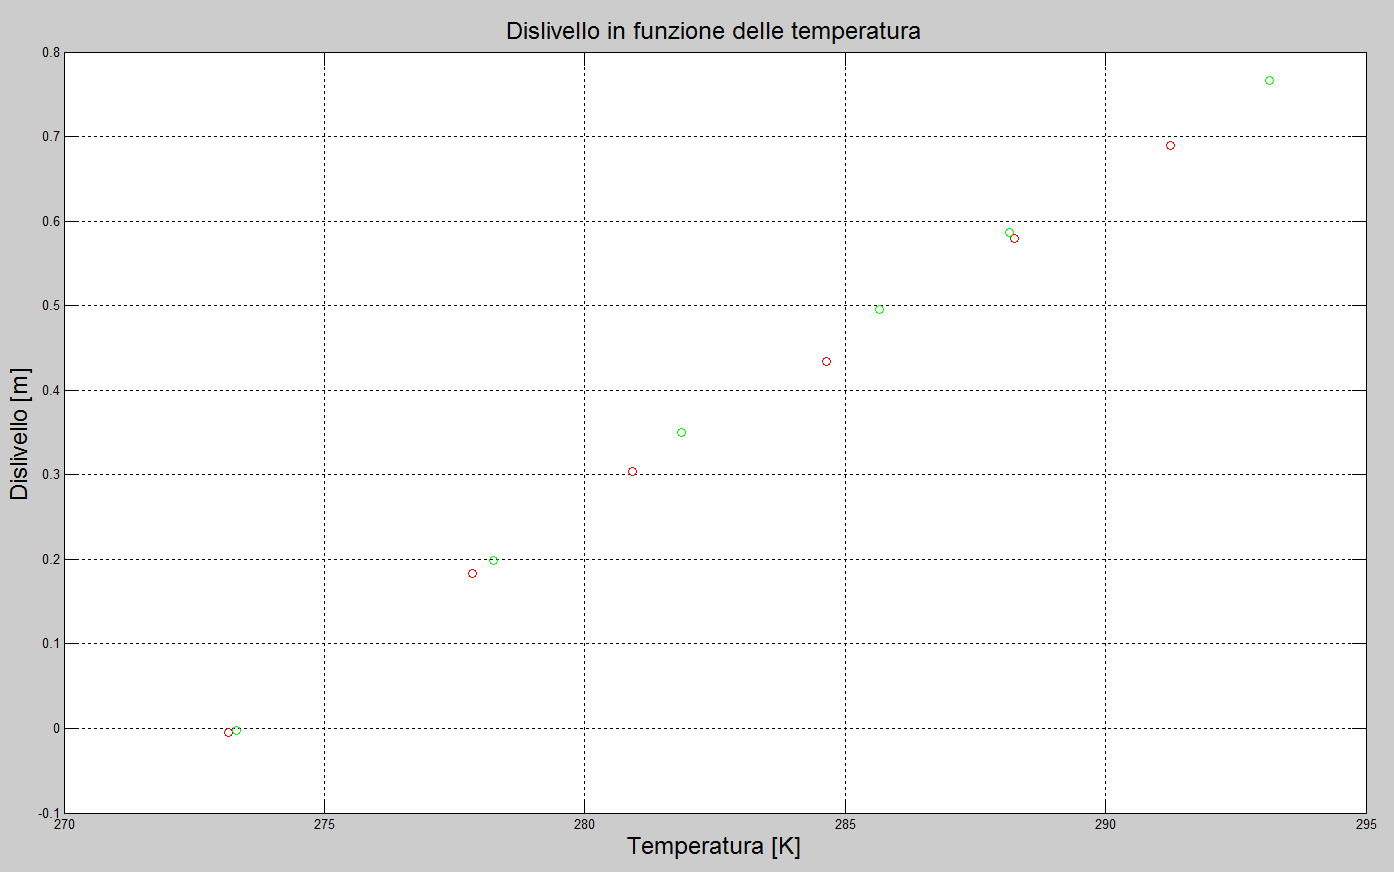
\includegraphics[width=\textwidth]{img/1}
\caption{Grafico di $\Delta h$ in funzione di $T$: scegliamo di rappresentare in colore rosso i dati riportati in Tabella 1.a ed in colore verde i dati riportati in Tabella 1.b}
\end{figure}

Tramite regressione lineare troviamo la retta $h = A+B\theta$ che meglio interpreta i nostri dati. 
Le formule per il calcolo sono la \eqref{eq:a} e la \eqref{eq:b} riportate in appendice.
Verifichiamo la bontà di questo risultato tramite test del $\chi^2$. Ci viene un $\chi^2=boh$, troppo alto rispetto all'aspettativa di 9 gradi di libertà.
L'incertezza è quindi troppo piccolo. 
Ricalcoliamo a posteriori l'incertezza e discutiamone la plausibilità.\\

\subsection{Determinazione dello \emph{zero assoluto}}
Durante l'esperienza si è utilizzato un barometro in laboratorio per la misura della pressione atmosferica $P_A$ variabile nel tempo. Nel nostro manometro differenziale la pressione dovuta alla colonnina di acqua è data da: $\Delta P = \rho gh$. 
La pressione $P$ del nostro gas è quindi 
\begin{equation}
\label{eq:p}
P = P_A + \rho gh
\end{equation}
In appendice B è riportata la Tabella relativa alla pressione atmosferica misurata nel tempo, grazie a quella e all'equazione \eqref{eq:p} possiamo stimare la pressione $P$ del gas in funzione della temperatura.\\
Stima delle incertezze\\
\begin{table}[H]
	\centering
	\begin{tabular}{|c|c|} \hline
		\textbf{P {[Pa]} } & \textbf{T {[\degree C]} }  \\ \hline
		 &   \\ \hline
		 &   \\ \hline
		 &   \\ \hline
		 &   \\ \hline
		 &   \\ \hline
		 &   \\ \hline
		 &   \\ \hline
		 &   \\ \hline
		 &   \\ \hline
		 &   \\ \hline
		 &   \\ \hline
	\end{tabular}
	\caption{Pressione del gas $P$ in funzione della temperatura $T$}
\end{table}

Da inserire in grafico :)


Lo zero assoluto è rappresentato graficamente dall'intersezione tra la retta del dislivello $\Delta h$ in funzione della temperatura $T$ e l'asse delle ascisse.
Questo punto rappresenta la condizione $P = 0$.
